\documentclass[10pt,a4paper,landscape]{article}

\usepackage{multicol}
\usepackage{calc}
\usepackage{ifthen}
\usepackage[landscape]{geometry}
\usepackage{hyperref}
\usepackage{lipsum}
\usepackage{graphicx}
\usepackage{amsmath}
\usepackage{amsfonts}
\usepackage{mathstyle}
\usepackage{mathtools}
\usepackage{commath}
\usepackage{enumitem}
\usepackage{siunitx}
\usepackage{fancyhdr}
\usepackage{extramarks}
\usepackage{titlesec}
\usepackage{listings}
\usepackage{amssymb}
\usepackage{bm}
\usepackage[usenames,dvipsnames]{color}
\usepackage{subfig}
\usepackage{booktabs}
\usepackage{float}
\usepackage{comment}

% Margin settings

\ifthenelse{\lengthtest { \paperwidth = 11in}}
	{ \geometry{top=0.2in,left=0.2in,right=0.2in,bottom=0.2in} }
	{\ifthenelse{ \lengthtest{ \paperwidth = 297mm}}
		{\geometry{top=0.2cm,left=0.2cm,right=0.2cm,bottom=0.2cm} }
		{\geometry{top=0.2cm,left=0.2cm,right=0.2cm,bottom=0.2cm} }
	}

% Turn off header and footer
\pagestyle{empty}

% Redefine section commands to use less space
\makeatletter
\renewcommand{\section}{\@startsection{section}{1}{0mm}%
                                {-1ex plus -.5ex minus -.2ex}%
                                {0.1ex plus .2ex}%x
                                {\normalfont\tiny\bfseries}}
                                % {\normalfont\large\bfseries\sc}}
\renewcommand{\subsection}{\@startsection{subsection}{2}{0mm}%
                                {-1explus -.5ex minus -.2ex}%
                                {0.1ex plus .2ex}%
                                {\normalfont\tiny\bfseries}}
\renewcommand{\subsubsection}{\@startsection{subsubsection}{3}{0mm}%
                                {-1explus -.5ex minus -.2ex}%
                                {0.1ex plus .2ex}%
                                {\normalfont\tiny\bfseries}}
\makeatother

\setlength{\parindent}{0pt}
\setlength{\parskip}{0pt plus 0.5ex}

% Some useful definitions
\def\*#1{\mathbf{#1}}
\def\L{\mathcal{L}}
\def\N{\mathcal{N}}

\usepackage{enumitem}
\setlist{leftmargin=10pt,topsep=0pt,itemsep=-1ex,partopsep=1ex,parsep=1ex}
\def\labelitemi{--}

% -----------------------------------------------------------------------


% Definitions of a dynamic environment for writing mathematical statements
% The margins used for this environment are different on the summary and the cheatsheet
\makeatletter
\renewenvironment{align*}{%
  \setlength{\abovedisplayskip}{3pt}%
  \setlength{\belowdisplayskip}{3pt}%
  \start@align\@ne\st@rredtrue\m@ne
}%
{\endalign}

% This environment only display content in the summary
\newenvironment{notImportant}
\makeatother

% Comment the "notImportant" sections 
\excludecomment{notImportant}

\newenvironment{Figure}
  {\par\medskip\noindent\minipage{\linewidth}}
  {\endminipage\par\medskip}

\begin{document}

\raggedright
\footnotesize

% Default itemize uses triangle
\renewcommand\labelitemi{$\triangleright$}
\renewcommand\labelitemii{$\triangleright$}

\begin{multicols*}{4}

% multicol parameters
% These lengths are set only within the two main columns
\setlength{\columnseprule}{0.25pt}
\setlength{\premulticols}{1pt}
\setlength{\postmulticols}{1pt}
\setlength{\multicolsep}{1pt}
\setlength{\columnsep}{2pt}

\begin{center}
     \small{\textbf{Mobile Network 2017 - Cheat Sheet}} \\
\end{center}

\tiny

% ==============================================================================

\section{Wireless communication and mobility}

\begin{notImportant}
	\begin{itemize}
		\item \textbf{user mobility}: users communicate "anytime, anywhere, with anyone"
		\item \textbf{device portability}: devices can be connected anytime, anywhere to the network
	\end{itemize}
\end{notImportant}

Wireless networks in comparison to fixed networks:

\begin{itemize}
	\item Higher data loss-rates due to interferences
	\item Restrictive regulations of frequencies
	\item Lower transmission rates
	\item Lower security, Higher jitter
	\item Fluctuation quality of the links
	\item Unknown location of the mobile station
\end{itemize}

% ==============================================================================

\section{Wireless Network Models}
Need to satify \textbf{coverage requirements} \& \textbf{service requirements}

Resources to be managed/conserved: \textbf{frequency spectrum}, \textbf{power consumption}, \textbf{infrastructure and terminal cost}

\textbf{Interference} often limites the performance of the system

\textbf{Technical measures} of a wireless network: number of subscribers served, overall bandwidth provided, BER, delay, user data rate, coverage, outage probability, ...

\textbf{Common Service types}
\begin{itemize}
	\item \textbf{Best Effort traffic}: guarantee maximum throughput. Utilize all available throughput at any time
    \item \textbf{Guaranteed service traffic}: constant data rate and delay
\end{itemize}

Network/infrastructure deployment: how many, where, what infrastructure and how much spectrum?

\textbf{Radio Resources allocation}: Given a set of base stations, allocate spectrum, power, ...

\textbf{Interference Models}: Propagation conditions on link $(i,j)$ given by $G_{ij}$ where $G$ is the link gain matrix.

\textbf{SINR} of uplink, downlink:
\begin{align*}
	\Gamma^u_{i_0 j} &= \frac{P_j G_{i_0 j}}{\sum_{m \neq j} P_m \theta_{0, m} G_{i_0 m} + N_{i_0}} \\
	\Gamma^d_{i_0 j} &= \frac{P_{i_0} G_{i_0 j}}{\sum_{b \neq i_0} P_b \theta_{0, b} G_{i_0 b} + N_{j}}
\end{align*}
with $\theta$ the normalized cross-correlation term.

Guaranteed service quality $\rightarrow$ boundaries on $\Gamma^u_{i_0 j}$ and $\Gamma^d_{i_0 j}$

$M$ terminals active, $Y$ terminals served, $Z = M - Y$ assignment failure.

\textbf{Assignment failure rate}: 
\begin{align*}
	v = \frac{E[Z]}{E[M]} = \frac{E[Z]}{ \omega A }
\end{align*}
with $\omega$ the terminal per unit area and $A$ the area.


\textbf{Capacity}: the maximum allowed traffic load in order to keep the assignment failure rate below some threshold.

\textbf{Resource Management Strategies}
\begin{itemize}
	\item \textbf{Static assignment}: based on statistical information during planning phase of the network
	\item \textbf{Perfect dynamic channel assignment}: based on instantaneous values. Traffic and interference adaptive assignment
	\item \textbf{Random assignment}: DS-CDMA, ALOHA, ...
\end{itemize}

% ==============================================================================

\section{Medium Access Control}

MAC protocols handle channel sharing between multiple terminals.

\textbf{Challenges for wireless networks}
\begin{itemize}
	\item Signal experiences reflection, diffraction, ...
	\item Broadcast nature of the medium
	\item Half-duplex: sending data usually prevents receiving
\end{itemize}

\textbf{Performance Measures}
\begin{itemize}
	\item \textbf{Delay}: between arrival time and time the message sent to receiver
	\item \textbf{Quality} of data received: 
	\begin{itemize}
		\item \textbf{BER}: Bit Error Ratio
		\item \textbf{$p_{BER}$}: Bit Error Probability
		\item \textbf{Packet Error Rate} $= 1 - (1 - p_{BER})^N$ 
	\end{itemize}
	\item \textbf{Throughput}: expected number of messages delivered to the receiver per time unit.
	\item \textbf{Normalized link delay}: 1 / throughput
\end{itemize}

% ------------------------------------------------------------------

\subsection{Contention-free MAC protocols}
Each terminal sends packets using predetermined time slots, frequency bands, or codes. A central scheduler coordinates the transmissions of different terminals, and \textbf{there will be no collisions} in the network.

\begin{notImportant}
	Pros and cons:
	\begin{itemize}
		\item[+] Appropriate for QoS guarantee
		\item[+] Works also with heavily loaded networks
		\item[-] Dynamic schemes have high complexity
	\end{itemize}
	Wireless resources can be divided into orthogonal partitions called \textbf{channels} and these can be assigned to different terminals.
\end{notImportant}

\textbf{Static resource partitioning}

\subsubsection{TDMA - Time Division Multiple Access}
\begin{itemize}
	\item All terminals are synchronized
	\item Flexible in handling different rate requirements
\end{itemize}
\subsubsection{FDMA - Frequency Division Multiple Access}
\begin{itemize}
	\item Not efficient for traffic with different rate requirements
	\item Need guard bands between adjacent bands $\rightarrow$ lower thrghput 
\end{itemize}
\subsubsection{OFDMA - Orthogonal Division Multiple Access}
\begin{itemize}
	\item Like FDMA but uses orthogonal sub-carriers
	\item Doesn't need guard band between adjacent frequency bands
	\item Allows overlapping adjacent spectrum bands $\rightarrow$ more spectrum efficient
	\item Easy to implement and used in 4G
\end{itemize}
\subsubsection{CDMA - Code Division Multiple Access}
\begin{itemize}
	\item Terminals send on whole frequency bandwidth
	\item Each sender has a unique code $\rightarrow$ XOR the signal with it
	\item[-] Higher complexity of the receiver
	\item[-] All signals should have the same strength at the receiver
	\item[+] Huge code space compared to frequency space
	\item[+] More robust to jamming and eavesdropping
	\item Used in 3G and Wifi
\end{itemize}
\subsubsection{SDMA - Space Division Multiple Access}
\begin{itemize}
	\item Uses the spatial separation to reuse frequency spectrum
	\item Useful when terminals are located far from each other
	\item Use intelligent signal processing and antenna arrays so it can reuse frequency spectrum within the same cell.
	\item Often combined with other partitioning methods.
\end{itemize}

\textbf{Dynamic resource partitioning} \\
Network resources can be dynamically allocated using a central scheduler to achieve better network performance. 
\begin{itemize}
	\item[+] Good performance in heavy traffic
	\item[+] QoS guarantee
	\item[-] Higher complexity and cost
	\item[-] Not scalable
\end{itemize}
\subsubsection{Poll-based access protocol}
\begin{itemize}
	\item Designate device as a channel access administrator
	\item Admin queries other terminals to see if they have packets
	\item If so, they transmit packets in the following several time slots
	\item Higher overhead as polling consumes a lot of bandwidth and turnaround time increases time overhead.
\end{itemize}
\subsubsection{Token-based access protocol}
\begin{itemize}
	\item Token is passed in a orderly fashion between the terminals.
	\item Terminal holding the token has the channel access.
\end{itemize}
\begin{notImportant}
	\begin{figure}
	    \centering
	    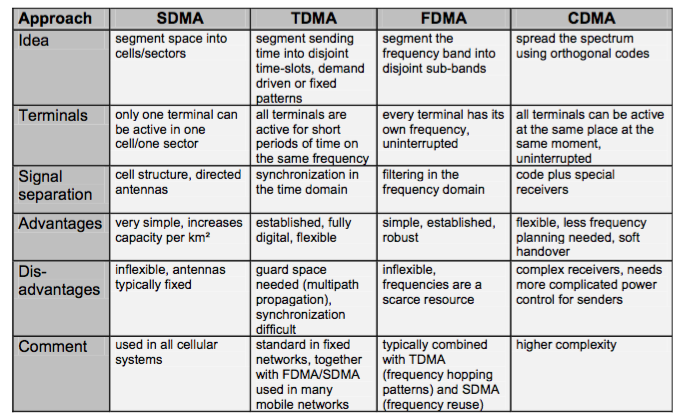
\includegraphics[width=.99\linewidth]{img/contentionfree}
	 \end{figure}
\end{notImportant}
% ------------------------------------------------------------------
\subsection{Contention-based MAC protocols}
\begin{itemize}
	\item Terminals access channel randomly when they have packets to send.
	\item No terminals is superior to another station
	\item Terminals decide when to send based on a procedure defined by the protocol
	\item Allows packet collisions
	\item[+] Good performance in low-traffic networks
	\item[+] Low complexity
\end{itemize}
\subsubsection{Pure ALOHA}
\begin{enumerate}
	\item If there is a message to send, send it
	\item 
	\begin{itemize}
		\item If the transmission succeeded $\rightarrow$ step 1
   		\item If the transmission failed, wait a random time $\rightarrow$ step 1
	\end{itemize}
	\item[$\triangleright$] Poor performance with high traffic
\end{enumerate}
\subsubsection{Slotted ALOHA}
\begin{itemize}
	\item Terminals are synchronized and can send packets only at the beginning of a time slot
	\item The average number of messages arriving to the system has to be equal to the average number of departing messages.
	\item Mathematical model
	\begin{itemize}
		\item $M$: \# terminals
		\item $\lambda_i = \lambda / M$: message arrival rate
		\item $\sigma_i$: message retransmission rate
		\item $\delta_i = \lambda_i + \sigma_i$: message attempt rate
		\item $q = e^{-M \delta_i}$: successful transmission probability
		\item $ \Rightarrow \lambda_i = q \delta_i$: for stable equilibrium
		\item $p = 1 - e^{-\delta_i}$: transmission probability
		\item Overall network thrghput:
		\begin{align*}
			\lambda = \sum_{i=0}^M \lambda_i = M \delta_i e^{-M \delta_i}
		\end{align*}
	\end{itemize}
\end{itemize}
\subsubsection{CSMA - Carrier Sense Multiple Access}
\begin{itemize}
	\item Abort transmission as soon as a collision is detected
	\item \textbf{Non-persistent CSMA}:
	\begin{enumerate}
		\item If the channel is sensed idle $\rightarrow$ send
    	\item Otherwise $\rightarrow$ wait a random amount of time and  $\rightarrow$ step 1
	\end{enumerate}
	\item \textbf{1-persistent CSMA}:
	\begin{enumerate}
		\item If the channel is sensed idle $\rightarrow$ send
    	\item Otherwise sens until idle $\rightarrow$ send
	\end{enumerate}
	\item \textbf{p-persistent CSMA}:
	\begin{enumerate}
		\item If the channel is sensed idle $\rightarrow$ send with prob $p$
		\\ Otherwise  $\rightarrow$ delay its transmission by one time slot
		\item If channel busy  $\rightarrow$ continue sensing until idle $\rightarrow$ step 1
	\end{enumerate}

\end{itemize}
\subsubsection{CSMA/CD - with Collision Detection}
\begin{itemize}
	\item If collision during transmission $\rightarrow$ stop and signal collision
	\item If collision occurs several time $\rightarrow$ increase time window (exp)
	\item \textbf{Not appropriate for wireless networks}
	\item \textbf{Hidden Terminal Problems}: Senders sense idle  but receiver in the middle get both messages at the same time.
	\item \textbf{Exposed Terminal Problem}: Senders sense channel busy while the receivers actually isolated
\end{itemize}
\subsubsection{CSMA/CA - with Collision Avoidance}
\begin{enumerate}
	\item At new transmission $\rightarrow$ choose backoff counter randomly
	\item Sense the channel: 
	\begin{itemize}
		\item if idle for DIFS (Duration Inter-Frame Space) $\rightarrow$ step 3 
		\item Otherwise $\rightarrow$ continue sensing
	\end{itemize}
	\item Count down using backoff counter while channel remains idle. 
	\begin{itemize}
		\item If the channel sensed busy $\rightarrow$ step 2. 
		\item If the counter is zero $\rightarrow$ transmit data immediately.
	\end{itemize}
	\item[$\triangleright$] \textbf{Request To Send (RTS)}, \textbf{Clear To Send (CTS)} packets, carrying data length solve exposed \& hidden terminal issue
\end{enumerate}
\subsubsection{CRA - Conflict Resolution Algorithms}
Resolves conflicts $\rightarrow$ users are scheduled using distributed algo.
\begin{itemize}
	\item Each terminal is uniquely numbered
	\item When conflict occurs $\rightarrow$ enters \textit{conflict resolution mode} until the conflict has been resolved $\rightarrow$ check last digit on IDs
\end{itemize}
\subsubsection{Reservation-Based Protocols}
\begin{itemize}
	\item Very costly to loose one long data packet when collision
	\item Reserve resources (time, frequency, ...) for data transmission
	\item Two phases: 1. reservation phase, 2. data transmission phase
	\item \textbf{Scheduling-based}: Central scheduler first collects networks information and then schedule the resources
	\item \textbf{Contention-based}: Short reservation pckt w/ ALOHA, CRA
\end{itemize}
\subsubsection{Bit-map protocol}
\begin{itemize}
	\item Terminals are numbered
	\item Send short reservation packet in the corresponding time slot
	\item Send data in the data phase folling order in resrvation phase.
	\item Station see all 1-bits resrvation transmitted during resrvation phase. Station know which stations want to transmit.
	\item After the resrvation phase, stations that asserted to transmit sends its frame in the order of station number.
	\item Efficiency: $\frac{d}{(d + N)}$, $d$ \# bits in the packet, $N$ \# terminals
\end{itemize}
\subsubsection{Bianchi's model}
\begin{itemize}
	\item Semi-analytical model to express performance of networks.
	\item Use 2D Markov C. of $m+1$ backoff stages in which each stage represent the backoff time counter of a node. Transitions take place upon collisions and successful transmissions
	\item In each stage, CW is the maximum value for the contention window and is equal to $2^i(CW_{min}+1)$
	\item If a correct transmission takes place, a random backoff will be chosen between $0$ and $CW_{0}-1$  with probability $\frac{1 - p}{CW_0}$ 
	\item In the case of a collision, a random backoff will be chosen between $0$ and $CW_{i}-1$ with probability $\frac{p}{C W_i}$
	\item State are represented as $\{s(t), b(t)\}$, $b(t)$: counter, $s(t)$: stage
	\item This model assumes that packets collide with probability $p$
	\item With $\pi$ the probability to send a packet: $p = 1 - (1 - \pi)^{N-1}$
	\item Stationary distribution of the chain:
	\begin{align*}
		b_{i,k} = \lim_{t \to \infty} P(s(t) = i, b(t) = k), i \in \{0, m\}, k \in \{0, CW_i - 1\}
	\end{align*}
	\item Transmission occurs when backoff time counter $=0$, therefore:
	\begin{align*}
		\pi = \sum_{i=0}^m b_{i,0}
	\end{align*}
	\item Close form of $b_{i,k}$
	\begin{align*}
		\left\{
			\begin{array}{c l l}
				b_{i,0} &= p^i b_{0,0} & 0 < i < m \\
				b_{m,0} &= \frac{p^m}{1-p} b_{0,0} \\
				b_{i,k} &= \frac{CW_i-k}{CW_i} b_{i,0} & 0 \leq i \leq m, 0 < k < CW_i-1
			\end{array}
		\right.
	\end{align*}
	Imposing normalization condition, we obtain $b_{0,0}$ as function of $p$:
	\begin{align*}
		b_{0,0} = \frac{2 (1 - 2p)(1 - p)}{(1 - 2p)(W_{min} + 1) + pW_{min}(1 - (2p)^m)}
	\end{align*}
	\begin{align*}
		\pi = \frac{b_{0,0}}{1 - p} = \frac{2}{1 + W_{min} + p W_{min} \sum_{k=0}^{m-1} (2p)^k}
	\end{align*}
	\item \textbf{Saturation throughput}: average information payload transmitted in a slot time over the average duration of a slot time:
	\begin{align*}
	\tau = \frac{P_s P_{tr} L}{P_s P_{tr} T_s + P_{tr} (1 - P_s) T_c + (1 - P_{tr}) T_{id}}
	\end{align*}
	with 
	\begin{align*}
		P_{tr} + 1 - (1-\pi)^N \text{ and } P_s = \frac{N \pi (1 - \pi)^{N-1}}{1 - (1 - \pi)^N}
	\end{align*}
	$T_{id}$: duration of the idle period, $T_c$: average time spent in collision, $T_s$: average time needed to transmit a packet of size $L$
\end{itemize}
% ==============================================================================
\section{Scheduling}
\begin{notImportant}
	Users have different service requirements so we need a flexible service architecture to intergrate different types of services on a single air-interface. Also, QoS metrics differ between different applications
\end{notImportant}

\subsection{Reservation-based access protocol w/ centr. sched.}
\begin{itemize}
	\item Most used access protocol in wireless cellular networks
	\item High efficiency and flexibility in managing wireless resources.
	\item \textbf{Physical Downlink Control Channel (PDCCH)}: \\
	$\rightarrow$ conveys control information for each user.
	\item \textbf{Physical Downlink Shared Channel (PDSCH)}: \\
	$\rightarrow$ multiplex the data of all terminals.
	\item Reservation phase: PDCCH. Data phase: PDSCH
	\item During the reservation phase, one can estimate channel and adapt scheduling in consenquence.
	\item Wireless scheduling suffers from \textbf{supporting a mix of classes} of traffic desiring different QoS.
	\begin{itemize}
		\item Conversational: Preserve time relation.
    	\item Streaming: Preserve time relation
    	\item Interactive: Request response pattern, preserve payload
    	\item Background: Destination is not expecting data within a certain time, preserve payload
	\end{itemize}
	\item \textbf{Channel Variation}: Channel is unstable, hard to predict, capacity of the link varies w.r.t. time and locations.
	\item Difficult to estimate the amount of resources needed. Thus, it is needed to use an adaptive procedure to assure QoS.
	\item For $M$ uplink users, the sum of the data rates is bounded
	\begin{align*}
		\sum_{i=1}^M r_i \leq W \log_2 
			\left(
				1 + \frac{\sum_i P_i g_{i0}}{N_0 W}
			\right)
	\end{align*}
	with $W$: frequency bandwidth, $P_i$: transmission power, $g_{i0}$: power gain of the channel and $N_0$: noise spectral density
	\item In the downlink, the base station sends independent data streams to multiple users.
	\item Assuming $g_{01} \leq g_{02} \leq ...$, the capacity region is:
	\begin{align*}
		r_m \leq W \log_2 
			\left(
				1 + \frac{P_m g_{0m}}{\sum_{i=m+1}^M P_i g_{0m} + N_0 W}
			\right) , \forall m
	\end{align*}
\end{itemize}
\subsection{Wireless Packet Scheduling Algorithms}
\begin{itemize}
	\item Increase flexibility in adaptation to QoS and channel
	\item Significant performance improvement
	\item Model contains M users served on a single channel, TDMA; each user has a buffer to store the packets to be sent.
	\item Queue modeling: At timeslot t, queue of user i updates: 
	\begin{align*}
		q_i[t+1] = q_i[t] + d_i[t] - n_i[t]
	\end{align*}
	$d_i[t]$: new bits arriving, $n_i[t]$: \# bits scheduled to transmit
\end{itemize}
$S_i$: long-run throughput for user $i$ can be predicted using
\begin{align*}
	\hat{S}_i[t] = (1 - \frac{1}{\tau}) S_i[t - 1] + \frac{1}{\tau} \hat{r}_i[t]I[i]
\end{align*}
where $\tau >> 1$ scheduler's constant, $\hat{r}_i$: expected data rate
\subsubsection{Round-robin scheduling}
\begin{itemize}
	\item One of the simplest scheduling algorithms
	\item Users are scheduled in round robin
	\item All users scheduled the same amount of resources
\end{itemize}
\subsubsection{Max throughput scheduling}
\begin{itemize}
	\item Schedule the minimal in each time slot $\rightarrow$ total network throughput is maximized.
	\item Most aggressive packet scheduler 
	\item[-] unfairness and coverage limitations. i.e. terminals in unfavorable positions may never be served.
\end{itemize}
\subsubsection{Proportional Fair Scheduling}
\begin{itemize}
	\item Compromised policy to balance the competing interests of maximizing total network throughput and providing all terminals with at least a minimum level of service.
	\item Meets the \textbf{Proportioanl fairness criterion} $\rightarrow$ When the scheduling result is already proportional fair, changing the scheduling such that the throughput of any user is increased by a percentage, the cumulative decrease of the throughputs of the other users will be higher.
\end{itemize}
\subsubsection{Max-Min Scheduling}
\begin{itemize}
	\item Objective: maximize the minimum user throughput
	\item Scheduling result is max-min fair iff increase of thrghput of one user results in decrease of a user with a smaller thrghput
\end{itemize}
\subsubsection{Max Utility Scheduling}
\begin{itemize}
	\item All previous schedulers do not consider QoS
	\item Utility $\equiv$ satisfaction of each user given allocated resources
	\item Model the QoS perception of users
	\item Objective: maximize the sum utility of all users
	\begin{align*}
		\max \sum_{i=0}^{M-1} U_i (S_i)
	\end{align*}
	\item Utility function determined based on traffic characteristics
	\item Different utility functions can be designed:
	\begin{itemize}
		\item Max-throughput: $U_i(S_i) = S_i$
		\item Proportional fair: $U_i(S_i) = \ln(S_i)$
		\item \textbf{Alpha Fair Utility}: Contains a parameter $a$ which mesures how fair the scheduler is. Get max throughtput when $a=1$ and is propotional fair when $a=0$
		\begin{align*}
			U_{\alpha}(S) = 
			\left\{ 
				\begin{array}{c l}
					\frac{S^{1 - \alpha}}{1-\alpha} & \alpha \geq 0 \text{ and } \neq 1 \\
					\ln(S) & \alpha = 0
				\end{array}
			\right.
		\end{align*}
	\end{itemize}
\end{itemize}
\subsubsection{Scheduling in OFDMA Systems}
\begin{itemize}
	\item One more dimension of resources: subcarrier allocation
	\item Different users experience: different gains because of frequency selectivity in channels
	\item Scheduling of subcarriers in an adaptive way based on the instantaneous channel qualities.
	\item Use adaptive subcarrier assignment, power allocation, modulation and coding to exploit the diversity in multiple users and frequency to improve the network performance.
	\item Usually combined w/ modulation and coding to improve perf.
	\item Additional signal overhead is necessary so the base station can inform all users the resource allocation results
	\item Round-robin, max-throughput, PF, max-min and max-utility scheduling can all be done for OFDMA
	\item \textbf{Power adaptation}: Each subcarrier should be assigned to the user with the highest Y (ratio between the channel gain and the interference) as the rate increase by using any amoung of power on any subcarrier will be maximized if the subcarrier has the hightest Y.
	\item Scheduling in OFDMA is usually based on optimization techniques to compute how much power should be used on each subcarrier. Generally no closed-form expressions.
	\item Expected overall throughput
	\begin{align*}
		R[t] = \sum_{i=1}^M R_i[t] = \sum_i \sum_j W \log_2 
			\left(
				1 + \frac{p_{ij}[t]y_{ij}[t]}{\theta}
			\right) \underbrace{I(i,j)}_{\text{assignement}}
	\end{align*}
	$y_{ij}[i]$: ratio between channel gain and interference
	\item Without power adaptation (max-thrput)
		\begin{align*}
			I^*(i,j) = 
				\left\{
					\begin{array}{c l}
						1 & \frac{p_{ij}[t]y_{ij}[t]}{\theta} \geq \frac{p_{mj}[t]y_{mj}[t]}{\theta}, \forall m\\
						0 & \text{otherwise}
					\end{array}
				\right.
		\end{align*}
	\item With power adaptation (max-thrput)
		\begin{align*}
			I^*(i,j) = 
				\left\{
					\begin{array}{c l}
						1 & y_{ij}[t] \geq y_{mj}[t], \forall m\\
						0 & \text{otherwise}
					\end{array}
				\right.
		\end{align*}
	\item Base station defines power allocation $p_{ij}$ to maximize thrput
\end{itemize}
% ==============================================================================
\section{Principles of cellular systems}
\begin{itemize}
	\item Cellular networks contain a set of fixed base stations
	\item Signal power decreasing with the distance $\rightarrow$ terminals connect to the closest base station
	\begin{align*}
		SNR = \frac{c_t P_t}{r^{\alpha} N}
	\end{align*}
	$r$: distance, $c_t$: antenna constant, $\alpha$: propagation constant 
	\item Considering \textbf{shadow fading} $\rightarrow$ received SNR becomes random - $G$ lognormal distribution. To preserve the same cell coverage area, need an extra \textbf{fade margin $M$} at the transmitter
	\begin{align*}
		P \left(
			\frac{c_t G P_t M}{r^{\alpha} N} \leq y_0
		\right)	\leq p_{out}
	\end{align*}
	\item W/ known radius, \# cells required to cover the service area is the ratio between total area and cell area.
	\item The \textbf{decibel}: dimensionless unit $\rightarrow$ power ratio. Express the magn. of a physical quantity relative to a reference level
	\item A value expressed in dB is computed as
	\begin{align*}
		10 \log_{10} (P/P_{\text{ref}})
	\end{align*}
	\item \textbf{Capacity of a wireless network (or radio capacity)} is measured as the average number of simultaneous radio links supported by the system.
	\item \textbf{Area capacity}: \# users per cell per unit area ratio.
	\begin{align}
		\text{area capacity} = (C/(K A_{\text{cell}}))
	\end{align}
	\item Trade off between quality (SINR) and capacity in the network \\
	$\rightarrow$ i.e.: with large clusters, the reuse distance is larger and thus the quality of the connections is increased
	\item Queueing modelling: \textbf{Blocking probability}
	\begin{align*}
		P_{block} = \frac{\rho^{\eta} / \eta!}{\sum_{k=0}^{\eta} \rho^{\eta}/k!}, \rho = \frac{\lambda}{\mu}
	\end{align*}
	\item Outage probability  $\equiv$ average over the pdfs of $t$
	\item \# assignment failures in a network with $n$ channels, $M$ mobiles is given by $Z = max(0, M-n) + Q$ with $Q$: \# mobiles having a channel but bad SINR
	\item \textbf{Assignment failure rate}:
	\begin{align*}
		v_p = \frac{E[Z]}{E[M_c]} = \sum_{k = \eta}^{\infty} (k - \eta) \frac{(\omega A_c)^{k-1}}{k!} e^{- \omega A_c}
	\end{align*}
	$\omega$ the number of calls (Poisson distributed) per unit area
	\item \textbf{Relative traffic load}:
	\begin{align*}
		\bar{\omega}_{\eta} = \frac{\omega A_c}{\eta}
	\end{align*}
	\item The system capacity can also be defined in terms of a combined blocking and signal outage, or \textbf{Grade of Service}
\end{itemize}

% Not essential
Other facts:
\begin{itemize}
	\item Cellular networks are based on efficient spectrum reuse
	\item Directional antennas reduce interference, improve coverage
	\item Cell capacity depends on the cell size 
	\item Small cells $\rightarrow$ better capacity
	\item Fading reduces the capacity of wireless networks
\end{itemize}

\begin{notImportant}
Design of wireless networks consists of two steps:
\begin{enumerate}
	\item Coverage planning
	\item Frequency allocation
\end{enumerate}
\end{notImportant}
\subsection{Coverage planning}
\begin{itemize}
	\item \textbf{Connection region} of a base station is the geometrical region where the received signal power from that base station is larger that from any other base station.
	\item \textbf{Coverage area} of each base station $\equiv$ \textbf{cell}.
	\item \textbf{Coverage planning problem}: find the required number of base s to be used with the servie area
	\item Common model used is uniform hexagonal-shaped areas
	\item It is pretty easy to compute the radius of the cells and \# of cells required to cover the service area
	\item channels / cells: $C$ available channels, K groups
	\begin{align*}
		\eta = \left \lfloor \frac{C}{K} \right \rfloor
	\end{align*}
	\item \textbf{Normalized reuse distance}
	\begin{align*}
		\frac{D}{R} = \sqrt{3K}
	\end{align*}
	with $R$ the radius, $D$ distance between cells
\end{itemize}
\subsection{Frequency Planning}
\begin{itemize}
	\item SINR at any receiver located in cell $k$
	\begin{align*}
		\Gamma_k = \frac{c \frac{P_t}{r^{\alpha}}}{\sum_{i=1...B} \frac{c P_t}{d^{\alpha}_i} + N}
	\end{align*}
\end{itemize}
\subsection{Static channel allocation}
\begin{itemize}
	\item \# simultaneous connections within the service area is often larger that \# orthogonal waveforms. $\rightarrow$ usefull to reuse same frequency within the service area as often as possible
	\item The higher the propagation loss as a function of distance, the more often we can reuse the spectrum
	\item \textbf{Reuse distance} is the minimum physical distance between two transmitters using the same waveform, required to achieve a certain link quality
	\item In \textbf{Fixed channel allocation (FCA)}, each access port is assigned a certain fixed number of channels. This allocation is achieved by dividing the C available channels into K (reuse factor) groups (clusters) of equal size. The access port has the right to use these channels freely to communicate with its terminals, but cannot use any channel from another group.
	\item To maintain a sufficiently high SINR, the channels in a group cannot be reused in a cell that is too close to the first cell
\end{itemize}
\subsection{Best-effort data services}
\begin{itemize}
	\item \textbf{bandwidth} of each channel: $W = W_s/K$
	with $W_s$ the total bandwidth
	\item \textbf{Instantaneous data rate} within a cell at distance $d = D/D_0$ from the base station
	\begin{align*}
	 	R(d) = \min(R_{max}, cW\log_2(1 + \Gamma(d)))
	 \end{align*} 
	 with $D_0$ the radius of the cell and $\Gamma(d) = \frac{\Gamma(D_0)}{d^{\alpha}}$
	 \item The data rate at the center of the cell is limited by peak rate $R_{max}$
\end{itemize}
\subsection{Directional antennas and sectorizations}
\begin{itemize}
	\item directional receiving antenna $\rightarrow$ reduce interference \\
	$\rightarrow$ $\downarrow$ the number of base station sites $\rightarrow$ $\downarrow$ infrastructure costs
\end{itemize}
% ==============================================================================
\section{More on cellular networks}
\subsection{Capacity of CDMA Cellular Networks}
\begin{itemize}
	\item Techniques to reduces interference:
	\begin{itemize}
		\item Multi-sectorized antennas
		\item Discontinuous transmission mode
	\end{itemize}
	\item \textbf{Power Control}: for a single cell, all uplink signals should be received $\approx$ with the same power at the base station
	\item \textbf{Pilot signal}: transmitted by the base station: used by each mobile to set its own power
	\item Average energy per bit, compared to noise power density:
	\begin{align*}
		\left(
		\frac{E_b}{I_0} 
		\right)_i = \frac{W}{R} \frac{G_{ii P_i}}{\sum_{k \neq i} G_{ki} P_k} + N_0 W = \frac{W}{T} \Gamma_i
	\end{align*}
	with $R= 1/ T_s$: data rate, $W$: interference bandwidth, $N_0$: additive noise power density.
	\item single cell case:
	\begin{align*}
		SNR = \frac{S}{(N-1)S} = \frac{1}{N-1}
	\end{align*}
	with $S$: power from single user, $N$: \# users
	\item bit energy to noise ratio
	\begin{align*}
		\frac{E_b}{N_0} = \frac{S/R}{(N-1)(S/W)} = \frac{W/R}{N-1}
	\end{align*}
	with $W$:available bandwith, $R$: bitrate, $N_0$: noise spectral density
	\item taking thermal noise $\eta$ into account
	\begin{align*}
		\frac{E_b}{N_0} = \frac{W/R}{(N-1) + (\eta / S)} \Rightarrow
		N = 1 + \frac{W/R}{E_b/N_0} - (\eta/S)
	\end{align*}
	\item To increase this number, switch off user while not talking and antenna sectorization:
	\begin{align*}
		\frac{E_b}{N_0} = \frac{W/R}{(N_s-1)\delta + (\eta / S)} \Rightarrow N_s = 1 + \delta 
			\left[ 
				\frac{W / R}{E_b / N_0}
			\right]
	\end{align*}
	with $N_s$: \# users per sector
\end{itemize}
\subsection{Femtocells}
\begin{itemize}
	\item Home base stations for mobile networks
	\item Licensed spectrum, low-power, low-range, better thrghput, better coverage, ...
	\item Susceptible to security attacks
\end{itemize}
\subsection{Frequency management}
\begin{itemize}
	\item In all countries of the world, the licensed spectrum is managed by the government and leased to private operators
	\item Auction or beauty contest based on very detailed dossiers
	\item Currently trying to allocate more frequencies for more bandwidth in mobile communication $\rightarrow$ a new total auction
	\item Mobile network is doubling every 9-12 mounths.
	\item Auctions is a transparent procedure and let the market determines the value of frequencies
	\item With auction of small frequency blocks, the market decides on the scope of the licences
	\item More rules to prevent people to abuse the auction
\end{itemize}
% ==============================================================================
\section{Association and Handover}
\begin{itemize}
	\item To each active terminal, in order to maximize system utility, we need to assign transmit power, waveform, base station
	\item Association on the move : \textbf{handover}
\end{itemize}
\subsection{Mobility management}
\begin{itemize}
	\item \textit{While inactive}: track the location of the terminal and wake it up when necessary (e.g. to update location area)
	\item \textit{While connected}: handover $\rightarrow$ timely selection of base stations based on signal quality measurements.
\end{itemize}
\subsection{Handover types}
\begin{itemize}
	\item \textbf{Involved networks}
	\begin{itemize}
		\item Horizontal handover: within a single network of homogeneous radio access technology (RAT)
    	\item Vertical handover: between different networks, heterogeneous RATs
	\end{itemize}
	\item \textbf{Hard handover}: only one base stations serving at a time
	\item \textbf{Soft handover}: multiple base stations can simultaneously serve a mobile terminal. Can lead to a better usage of radio resources, at the expense of higher complexity
\end{itemize}
\subsection{Handover phases}
\begin{enumerate}
	\item Measurement and decision
	\item Resource management 
	\item Execution (handshaking)
\end{enumerate}
\subsection{Performance metric}
\begin{itemize}
	\item Handover failure probability
    \begin{itemize}
    	\item Handover attempts fail
    	\item Prob. that signal quality is below the required value
    \end{itemize}
	\item Handover frequency
\end{itemize}
\subsection{Handover decision criteria}
\begin{itemize}
	\item Received signal strength (cell boudaries)
	\item Signal to interference ratio
\end{itemize}
\subsection{Handover resource management}
\begin{itemize}
	\item Resource reservation for handover
	\item Protection of ongoing services is more important than accepting new services
	\item Its significance depends on delay tolerance of the service
\end{itemize}
\subsection{Handover execution}
\begin{itemize}
	\item System and mobile should reach agreement on which base station to pass, which waveform, authentification, ... 
	\item Procedure has to be fast and reliable
\end{itemize}
\subsection{Load balancing}
\begin{itemize}
	\item Traffic load fluctuates a lot over time
	\item neighbor cell may have much lighter load at the moment
\end{itemize}
% ==============================================================================
\section{F-Transport}
\subsection{Reminder TCP}
\begin{itemize}
	\item Reliable, in-order packets delivery
	\item Single path
	\item Congestion avoidance and control
	\item Three-way handshake
	\item Lost packet detection using sequence numbers and ACKs
\end{itemize}
Nowadays, hosts have several interfaces, or multiple addresses for a single interface. Addresses of mobile hosts can change as they move from one network to another. Current TCP is not designed to switch between interfaces as they come and go.\\

\textbf{Link aggregation}: combine multiple channels at different frequencies and use different radio technologies into a single link


\subsection{Multipath TCP (MPTCP)}
MPTCP is a modification of TCP presenting regular TCP interfaces to applications, spreading data across several TCP subflows. Achieve higher throughput, failover from one path to another and seamless mobility.
\begin{itemize}
	\item First establish the intial subflow
	\item Then additional subflows can be established
	\item At least one of those need to differe between two subflows: Local IP, Remote IP, Local Port, Remote Port
	\item Use two levels of sequence numbers to prevent gaps in seq.
	\item Dseq: data sequence number (SQN) and seq is the additional SQN carried inside the TCP option. It ensures that the segments sent on any given subflow have consecutive SQNs.
	\item On linux, upon timeout expiration, re-evaluate whether packet could be retransmitted over another subflow
	\item Upon loss of a subflow, all the unacknowledged data are retransmitted on other subflows
\end{itemize}

\subsubsection{MPTCP Congestion Control}
\begin{itemize}
	\item Each path runs its own congestion control, detect, respond
	\item MPTCP send all its traffic on its least-congested paths
	\item Users get at least as much thrghput as w/ single-path TCP
\end{itemize}

% Not really relevant
\subsubsection{MPTCP Congestion Control Algorithm}
\begin{itemize}
	\item A connection consits of a set of subflows R
	\item Each subflow maintains a congestion window
	\item Specific rules on how to increase and decrease the windows
	\item Still experimental, but largely deployed on smartphones
\end{itemize}
% ==============================================================================
\section{Wireless Network Security}
\begin{itemize}
	\item In wireless networks, sending and receiving messages do not need physical access to the network
	\item Wireless communications have a broadcast nature, therefore, transmissions can be overheard by anyone in range
	\item Easy to, eavesdrop, replay messages, jamming, ...
	\item Security requirements
	\begin{itemize}
		\item Confidentiality: use encrypted messages
		\item Authenticity: origin of the message must be verified
		\item Replay detection
		\item Integrity: messages stay un-modified
		\item Access control: access provided only to legitimate entities
		\item Protection against jamming
	\end{itemize}
\end{itemize}
\subsection{Cellular Network Security}
\subsubsection{GSM (2G) - Global System for Mobile com.}
\begin{itemize}
	\item Provides subscriber authentication
	\item Uses long-term secret key to generate session keys
	\item Provides protection of the subscriber's identity from eavesdroppers
	\item Provides confidentiality of communications
	\item User devices have SIM card (Subscriber Identity Module)
	\begin{itemize}
		\item Allows to authenticate on the network
		\item Contains a secret key
		\item Encrypted with a PIN (Personal Identification Number)
		\item User permanent identity, \textbf{IMSI} (International Mobile Subscriber Identity)
		\item If possible don't use IMSI but temporary TMSI
	\end{itemize}
	\item weaknesses: 
	\begin{itemize}
		\item Unilateral authentication \\
		$\rightarrow$ fake base station can pretend to be legitimate network
		\item No security within the wired network
		\item Uses 1st generation of cryptography
		\item SIM cloning
	\end{itemize}
\end{itemize}
\subsubsection{UMTS (3G) - Universal Mobile Telecom. Systems}
\begin{itemize}
	\item Provides protection against false base stations
	\item Key lengths were increased $\rightarrow$ stronger encryption
	\item Security mechanism within the networks
	\item However no end-to-end encryption
\end{itemize}
\subsubsection{LTE (4G) - Long Term Evolution}
\begin{itemize}
	\item Even more secure
	\item Completely IP-based
	\item Security principles:
	\begin{itemize}
		\item Permanent security association with home network
		\item New key hierarchy
		\item Reciprocal authentication mechanisms
		\item Trusted environment (in isolation from the OS)
		\item DoS protection of the network
		\item User privacy
		\item Authorization required for connection to core networks
	\end{itemize}
\end{itemize}
\subsubsection{WEP - Wired Equivalent Privacy}
\begin{itemize}
	\item Before association, the station needs to authenticate itself
	\item Default key is manually installed in every station and the AP
	\item Default keys need to be changed when a member leaves the group, practically impossible to change in every device simultaneously
	\item hence, supports \textbf{multiple default keys}: message header contains a key ID, tells which key should be used for decryption
	\item Weaknesses:
	\begin{itemize}
		\item Authentication is one-way only
		\item Same key is used for authentication and encryption
		\item No session key is established during authentication
		\item No replay messages protection
		\item Broken authentication protocol
	\end{itemize}
\end{itemize}
\subsubsection{WPA/WPA2 - WiFi Protected Access}
\begin{itemize}
	\item Authentication process results in a shared session key
	\item Different functions use different keys
	\item Integrity protection is improved
	\item Weaknesses:
	\begin{itemize}
		\item Weak passwords
		\item TKIP (encryption algo) has been broken
		\item PIN can be bruteforced easily in 2 hours
	\end{itemize}
\end{itemize}
\subsubsection{Wireless Pairings}
\begin{itemize}
	\item Used when there is no central authority distributing keys
	\item Devices pair by themselves and set up keys
	\item Use symmetric key techniques or Diffie-Hellman
\end{itemize}
\subsubsection{Diffie-Hellman Protocol}
\begin{itemize}
	\item Enables secret key establishment in cleartext
	\item Fully resits passive attackers
	\item Not secure against active attackers, hence need authentication
	\item Based on the discrete logarithm problem:
	\begin{itemize}
		\item $A$ generates $a$, computes and send $(g^a \mod p)$. $B$ generates $b$, computes and send $(g^b \mod p)$. They can both generate the key
		\begin{align*}
			k = (g^b \mod p)^a = (g^a \mod p )^b
		\end{align*}
		with $p$ a prime number and $g$ a generator of $Z_p^*$
	\end{itemize}
\end{itemize}
\subsubsection{Other techniques}
\begin{itemize}
	\item \textbf{Short String Comparison}: Display hash of the key on the screen, visually compare 
	\item \textbf{Seeing is Believing}: Uses optical channel (in which impossible to perform MitM attack) to validate key exchange.
	\item \textbf{Loud and Clear}: Human-assisted string comparison using voice communication
	\item \textbf{Shake Them Up}: Rely on the fact that the attacker does not know which device transmits at which time
	\item \textbf{Integrity Regions}: Distance-bounding protocols (proved that devices are at most at X cm from each others)
\end{itemize}
\subsubsection{In practice}
\begin{itemize}
	\item Bluetooths's device pairing aims at creating one shared secret called the Link Key. This key is used both for authentication and encryption. Uses a PIN-based protocol called \textbf{Link Manager Protocol (LMP)}
	\item \textbf{Sound-Proof}: Sense ambient audio to verify proximity of the two devices
\end{itemize}

% ==============================================================================

\section{Privacy in Mobile Network}
\begin{itemize}
	\item \textbf{Privacy control}: ability of individuals to determine when, how, and to what extend information about themselves is revealed to others
	\item \textbf{Anonymity}: hiding who performed a given action
	\item \textbf{Untraceability}: making difficult for adversary to identify that given actions were performed by the same subject
	\item \textbf{Unlinkability}: hiding relationships between any item
	\item \textbf{Unobservability}: hiding of the items themselves
	\item \textbf{Pseudonymity}: use of a pseudo instead of real identity
	\item \textbf{Anonymity set}: subjects that might performed the action
	\item \textbf{Privacy metrics}: 
	\begin{itemize}
		\item \textbf{Anonymity set}: set of subjects that mights have performed the action
		\item Measure of anonymity:
		\begin{align*}
			- \sum_{\forall x \in A} p_x \log p_x
		\end{align*}
		$A$: anonymity set, $p_x$: prob. that $x$ performed the action
		\item Measure of unlinkability
		\begin{align*}
			- \sum_{\forall R \subseteq I_1 \times I_2 } p_r \log p_r
		\end{align*}
		$p_r$: prob real relationship between elements in $I_1$ and $I_2$
		\item Measure of certainty:
		\begin{align*}
			-\sum_{v \in V} p_v \log p_v
		\end{align*}
		$V$: set of possible values, $p_v$: prob that the value is $v$ for a given user
	\end{itemize}
\end{itemize}
\subsection{Location privacy}
\begin{itemize}
	\item With location-based services, users upload location episodically on network
	\item Use pseudo is a solution for the location privacy problem
	\item However changing pseudo at each timestamp is ineffective against a global eavesdropper (can predict your next location and infer the new pseudonym)
	\item \textbf{Mix zone}: unobserved zone where the vehicles change  pseudo 
	\item Vehicles do not know where the mix zone is \\
	$\rightarrow$ need to change pseudo frequently
	\item \textbf{Model of the mix zone}:
	\begin{itemize}
		\item $p_{ij}$: prob exiting at $j$ and entering at $i$
		\item $D_{ij}$: RV representing time that elapses between entering at $i$ exiting at $j$
		\item $d_{ij} = P(D_{ij} = t)$
		\item $P($ exit at $j$ at $t$ and enter at $i$ at $\tau) = p_{ij} d_{ij(t - \tau)}$
		\item each possible mapping between exit and enter events is represented by a permutation $\pi$:
		\begin{align*}
			m_{\pi} = (N_1 <> X_{\pi[1]}, ..., N_k <> X_{\pi[k]})
		\end{align*}
		\begin{align*}
			P(m_{\pi}, \bar{X} | \bar{N}) = \prod_{i=1}^k p_{n_i x_{\pi[i]}} d_{n_i x_{\pi[i]}} (t_{\pi[i]} - \tau_i) = q_{\pi}
		\end{align*}
		\begin{align*}
			H(\bar{N}, \bar{X}) = -\sum_{\pi} \frac{q_{\pi}}{\sum_{\pi'} q_{\pi'}} \log 
				\left( 
					\frac{q_{\pi}}{\sum_{\pi'} q_{\pi'}}
				\right)
		\end{align*}
	\end{itemize}
	\item \textbf{Tracking game}: adversary picks a vehicle in the obeserved zone. When this vehicle enters a mix zone, estimates time to enter other obvesable zones. When a vehicule enter obversable zone, compute probability of vehicle to be the one.
	\item Level of privacy is the success probability of the adversary
	\item \textbf{Location-Privacy Meter (LPM)}: open source software tool to quantify location privacy
	\item \textbf{Adversary model}: using observation and knowledge such as users' mobility profiles, the adversary can infer location by computing some probability distribution.
	\item \textbf{Inference Attack}: TODO -> uses de-anonymization and de-obfuscation
\end{itemize}
\subsection{IMSI catchers}
\begin{itemize}
	\item \textbf{IMSI}: International Mobile Subscriber Identity
	\item Fake mobile towers acting between the target mobile phone and the service provider's real towers
	\item Used to track users, eavesdropping calls, geotargeting ads
	\item Used by law enforcement and intelligence agencies
	\item Use lack of mutual authentication, lack of encryption in the current mobile network implementations (mainly GSM, 2G)
	\item We can catch them using the constant parameters broadcasted by the cell towers
\end{itemize}
% ==============================================================================

%\begin{notImportant}
	\section{Hands-On Exercise 1}
	\begin{itemize}
		\item \textbf{Distributed coordination function (DCF)} is the basic medium access mechanism of IEEE 802.11, and uses a CSMA/CA algorithm.
		\begin{itemize}
			\item Basic access method: is channel busy, a backoff time is randomly chosen in $[0, CW]$. This timer is decremented by one as long as the channel is sensed idle for a \textit{distributed inter frame space} $DIFS = SIFS + 2 \times SlotTime$. $CW$ is doubled after each unsuccessful transmission. When the backoff timer reaches zero, the source transmits the data packet. The ACK is transmitted by the receiver immediately after a period of time called \textit{short inter frame space} SIFS. When a packet is transmitted, all other stations hearing this transmission adjust their \textit{network allocation vector} NAV, maintaining a prediction of future traffic on the medium.
			\item Optional channel access method with \textit{request-to-send} RTS and \textit{clear-to-send} CTS exchanged.
		\end{itemize}
		\item \textbf{Point coordination function (PCF)} is a centralized, polling-based access mechanism which requires the presence of a base station that acts as an access point. An RTS frame should be transmitted by the source and the destination should accept the data transmission by sending CTS frame prior to the transmission of the actual data packet.
		%\item TODO Frame format
	\end{itemize}
%\end{notImportant}


% ==============================================================================






%\newpage

\begin{center}
     \small{\textbf{Exercices and Exams}} \\
\end{center}

\tiny

% ==============================================================================

\section*{HW 1}

\subsection*{Ex 1.1}
If two channels are mutually exclusive in terms of time, then the capacity of the link is 
\begin{align*}
	c = \frac{c_1 c_2}{c_1 + c_2}
\end{align*}

\subsection*{Ex 1.2}
For minimum acceptable SIR of 10 dB, with power la distance dependence model, solve the equation 
\begin{align*}
	\frac{S}{I} = \frac{c P_{t2} / d_2^{\alpha}}{c P_{t1} / d_{12}^{\alpha}} \geq 10
\end{align*}

\subsection*{Ex 1.4}
Given a gain matrix $G$ for two access ports and three terminals, apply uplink and downlink formula to compute the different throughputs for the different combination of assignment.

% ==============================================================================

\section*{HW 2}

\subsection*{Ex 2.1 - Slotted ALOHA}
Given arrival rate of packets modeled with a Poisson distribution
\begin{align*}
	P(k) = \frac{G^k e^{-G}}{k!}
\end{align*}
with $G$ the channel load and knowing $94\%$ of the slots idle:
\begin{itemize}
	\item Compute channel load: 
	\begin{align*}
		P(0) = e^{-G} = 0.94
	\end{align*}
	\item Compute throught of the system
	\begin{align*}
		S = P(1) = G e^{-G }
	\end{align*}
	\item Compute fraction of busy slots
	\begin{align*}
		1 - P(0)
	\end{align*}
	\item Compute fraction of busy slots with collisions amongs busy slots
	\begin{align*}
		\frac{1 - P(0) - P(1)}{1 - P(0)}
	\end{align*}
	\item Calculate peak throughtput
	\begin{align*}
		\frac{\delta S}{\delta G} = 0 \rightarrow e^{-G_{peak}} - G_{peak} e^{-G_{peak}} = 0  \Rightarrow S(G_{peak})
	\end{align*}
\end{itemize}

\subsection*{Ex 2.2}
$N$ stations on the same channels, transmit with probability $p$ at each time slot.
\begin{itemize}
	\item Throughput of the system
	\begin{align*}
		S = N p(1-p)^{N-1}
	\end{align*}
	\item Compute $p$ that maximizes the throughtput
	\begin{align*}
		\frac{\delta S}{\delta p} = 0 \rightarrow p = \frac{1}{N}
	\end{align*}
\end{itemize}

\subsection*{Ex 2.3}
Channel operating at 25 Mbps. $M$ workstations at 100 meters aways from the acces point. Polling messages are 64 bytes long and packets are of constant length of 1250 bytes. When no more packets to transmit, notification with a 64-byte message.
\begin{itemize}
	\item Compute maximum possible arrival rate (packets/secs) if stations are allowed to transmit unlimited number of packets per poll:
	\begin{align*}
		\lambda_{max} = \frac{N}{T_{tot}}
	\end{align*}
	with
	\begin{align*}
		T_{tot} = N \times T_{packets} + T_{poll} + T_{end} + 2 t_{prop}
	\end{align*}
	with $N$ the number of packets allowed to transmit and $t_{prop}$ the propagation time. Given light speed $c$ and distance $d$
	\begin{align*}
		t_{prop} = d / c
	\end{align*}
	Then
	\begin{align*}
		N \rightarrow \infty \Rightarrow \lambda_{max} = \frac{1}{T_{packet}}
	\end{align*}
\end{itemize}

\subsection*{Ex 2.4 - Frame headers - TODO}

\subsection*{Ex 2.5 - Timing diagram CSMA-CA - TODO}


% ==============================================================================

\section*{HW3}

\begin{notImportant}
\subsection*{Ex 3.1 - Proportional Fare Scheduler}
Denot $M$ the number of terminals, $S_i$ the long-run throughput of terminal $i$, the scheduler tries to maximize:
\begin{align*}
	\sum_{i=0}^{M-1} \ln S_i
\end{align*}
TODO proof
\end{notImportant}

\subsection*{Ex 3.2.1 - Network throughput}
TDMA system with 4 terminals and data rate $R_i$.
\begin{itemize}
	\item Compute throughput with \textbf{Max-min scheduling}:\\
	Try to assigns time slots such that 
	\begin{align*}
		x_i r_i = x_j r_j
	\end{align*}
	with $x_i$ the percent of the slots and $r_i$ the data rate. Each terminal will have same throughput so its easy to compute the total throughput $S$.

	\item Compute throughput with \textbf{Round-robin scheduling}:\\
	Each terminal we be assign the same percent of the slots. Easy to compute $S$.
\end{itemize}

\subsection*{Ex 3.2.2}
Two terminals scheduled bu prop. faire scheduler. Rates are 64 and 128 kbps. The transmission continues for 2 time slots and $S_1[1] = 64$, $S_2[1] = 128$. The average throughput is update as follow:
\begin{align*}
	S_i[t] = (t-1)/t \times S_i[t-1] + 1/t \times \hat{r}_i[t] i[t]
\end{align*}
Calculate the average throughput of each terminal:\\
In the first slot
\begin{align*}
	i[1] = \arg \max_i(\frac{64}{64}, \frac{128}{128}) = 1 \text{ or } 2
\end{align*}
Both terminals can be schedule. Suppose terminal 1 is selected, then update and compute $S_1[2], S_2[2]$. Update 
\begin{align*}
	i[2] = \arg \max_i(\frac{64}{64}, \frac{128}{64}) = 2
\end{align*}
Update and compute $S_1[3]$ and $S_2[3]$.

\subsection*{Ex 3.3 Bianchi model TODO}


% ==============================================================================

\section*{HW 4 - Principles of Cellular Systems}

\subsection*{Ex 4.1}
System with $C$ channels and minimum SIR of 19 dB using symmetric hexagonal plan. $D$ is the distance between centers of nearest co-channel cells. $R$ is the radius of a cell. 6 co-channels for each distances $\sqrt{3} D, \sqrt{4}D, ... \sqrt{(i+j)^2 - ij} D$. Assume propagation model $P_r = c P_t d^{\alpha}$ and all stations transmi with power $P$.
\begin{itemize}
	\item Find expression for co-channel interference on downlink channel: \\
	\begin{align*}
		\Gamma_A    &= \frac{\frac{cP}{R^{\alpha}}}{6 \times (\frac{cP}{D^{\alpha}} + \frac{cP}{(\sqrt{3}D)^{\alpha}} + ...)} \\
					&= \left( \frac{D}{R}\right)^{\alpha} \frac{1}{6 \times (1 + \frac{1}{3^{\alpha/2}} + ... )}
	\end{align*}
	The sum at the denominator doesn't converge for $\alpha \Rightarrow \Gamma_A = 0$. In practice $\alpha > 2$ dut to obstables, fading, ...

	\item Compute the \textbf{radio capacity} $\eta$ of this system for $\alpha = 4$: \\
	We know that 
	\begin{align*}
		K = \frac{1}{3} (\frac{D}{R})^2
	\end{align*}
	So using the previous result
	\begin{align*}
		\Gamma_A = \left( \frac{D}{R}\right)^4 C \geq 10^{1.9} (19 dB) \Rightarrow K \geq \sqrt{\frac{10^{1.9}}{9 C}} 
	\end{align*}
	Also, given the symmetric hexagonal cell plan, $K$ has to satisfy $K = (i+j)^2 - ij$. We can then compute $K$ and $\eta$. 
\end{itemize}

\subsection*{Ex 4.2 - Sectoring technique}
We only consider the first tier of interferers (distance $D$). We have $K = 7$ and minimum SIR at 18.45 dB.
\begin{itemize}
	\item Show that the system satisfies minimum requirement:
	\begin{align*}
		\Gamma_A = (\frac{D}{R})^4 \frac{1}{6} = \frac{3 K^2}{2} > 10^{1.845}
	\end{align*}
	\item Use directional antennas dividing each cell into three sectors (120'). Compute radio capacity: \\
	Reduce number of co-channel interferes from 6 to 2. Therefore
	\begin{align*}
		\Gamma_A = (\frac{D}{R})^4 \frac{1}{2} \geq 10^{1.845} \Rightarrow K = \frac{1}{3} \sqrt{2 (\Gamma)} \Rightarrow \eta = \left \lfloor \frac{C}{K} \right \rfloor
	\end{align*}
	The result is nearly twice the capacity of the system with omni-directional antennas.
\end{itemize}


% ==============================================================================

\section*{H5 - Association and Handover}

\subsection*{Ex 5.1}
Assume straight highway of 8km with traffic density
\begin{align*}
 	\rho(x) = 
 		\left\{
 			\begin{array}{c l}
 				x^2 & \text{ if } 0 \leq x \leq 2 \\
 				4 - \frac{x}{2} & \text{ if } 2 \leq x \leq 8 \\
 				0 & \text{ otherwise} 
 			\end{array}
 		\right\}
 \end{align*} 
 and we are deploying two base stations covering the highway.
 \begin{itemize}
 	\item Assume $0 \leq z \leq 2$ ($z$ the handover point), show that we can't distribute traffic load between the two stations: \\
 	Traffic load on both side should be equal: $\lambda_1 = \lambda_2$, we have
 	\begin{align*}
 		\lambda_1 = \int_0^z x^2 \: dx = \lambda_2 = \int_z^2 x^2 \: dx + \int_2^8 (4 - \frac{x}{2}) \: dx
 	\end{align*}
 	Solving this we have $z = 2.6 > 2$.

 	\item Find best location $y$ for the right base station. We want to keep the overall power radiated to a minimum. To estimate the weight of the traffic of all terminals at both sides of the base station, we can integrate the product of the traffic intensity function and the square of the distance from $y$. We want the weights on both side to be equal.
 	\begin{align*}
 		w_1 = \int_z^y (4-\frac{x}{2})(y-x)^2 \: dx = w_2 \int_y^8 (4-\frac{x}{2})(y-x)^2 \: dx
 	\end{align*}
 \end{itemize}

% \subsection*{Ex 5.2} Not relevant

% ==============================================================================

\section*{HW 6 - Transport Layer}

\subsection*{Ex 6.1 - Sequence numbers in MPTCP}
\begin{itemize}
	\item Why a single sequence space is not enough in MPTCP: Because striping seq numbers across two paths will leave gaps in the sequence space seen on any single path. Some network middleboes will not allow a gap in sequence numbering space.
	\item TODO - illustration
\end{itemize}

\subsection*{Ex 6.2 - Congestion control in MPTCP}
In MPTCP, connection consists of a set of subflows $r \in R$, with each their own congection window $w_r$. $RTT_r$ the round trip time on subflow $r$. For each ACK on subflow $r$ compute 
\begin{align*}
	\min_{S \subseteq R: r \in S} \frac{\max_{s \in S} w_s / RTT^2_s}{(\sum_{s \in S} w_s / RTT_s)^2}
\end{align*}
then find the minimum and increase $w_r$ by that much. \\
For each loss, decrease $w_r = w_r /2$

\begin{itemize}
	\item What if each subflow was just running a regular TCP congestion control algorithm: It would be unfaire because MPTCP connections would get much more throughput than single path TCP.

	\item If only one subflow, behaves like regular TCP (super obvious)
\end{itemize}

% ==============================================================================
\section*{HW 7 - Security}

\subsection*{Ex 7.1}
\begin{itemize}
	\item Symmetric-key encryption: confidentiality, Authentication
	\item Asymmetric-key encryption: Confidentiality
	\item Hash functions: Data integrity, Authentication
	\item MACs: Data integrity, Authentication -> hash the data and include it in the message. Reciever can recompute MAC and check data integrity.
	\item Digital signatures: Data integrity, Authentication, Non-repudiation
\end{itemize}

\subsection*{Ex 7.2 - Diffie-Hellman}
\begin{itemize}
	\item \textbf{Key agreement protocal}: when both participants contribute information to the established key
	\item If non of the participtans knows the verification algorithm of the other, then an man-in-the-middle attack is possible.
	\item TODO
\end{itemize}

\subsection*{Ex 7.3 - GSM security}
\begin{itemize}
	\item In GSM security, why does the mobile station use 2 different keys (user's secret and ciphering key)?:\\
Using secret key too often leaks some information about this key. Therefore it uses long-term secret key to generate a session ciphering key and use this new key to encrypt the data.

	% TODO \item Why sending $R$ to the mobile station?
\end{itemize}

\subsection*{Ex 7.4}
How can a rogue base station establish a session in GSM: \\
In GSM, only the mobile authenticates to the visited network. The rogue station only needs to reply with a random number after the authentication procedure by sending the IMSI number. Using crypto-analysis, the rogue station could infer the secret key of the mobile (might take a while)

% TODO \subsection*{Ex 7.5}

% ==============================================================================

\section*{HW 8 - Privacy protection}
Consider a mix zone with $n \geq 2$ ports in which the transition probabilities $p_{i,j}$ (exiting at $j$ when entering at $i$) are $\frac{1}{n}$. At time 0, 2 cars enter the mix-zone at ports 1 and 2 at time $t_1$ and $t_2$.
\begin{itemize}
	\item Quantify the uncertainty of the adversary regarding the mapping between enter and exit event for the folloring distribution of the time spent in the mix-zone:
	\begin{align*}
		d_{1,1}(t_1) = 0.5, d_{1,2}(t_2) = 0.25, d_{2,1}(t_1) = 0.5, d_{2,2} = 0.5
	\end{align*}

	For event $(1 \rightarrow 1, 2 \rightarrow 2)$ we have likelihood: 
	\begin{align*}
		p_{1,1}d_{1,1} \times p_{2,2}d_{2,2} = \frac{1}{4 n_2}
	\end{align*}

	For event $(1 \rightarrow 2, 2 \rightarrow 1)$ we have likelihood: 
	\begin{align*}
		p_{1,2}d_{1,2} \times p_{2,1}d_{2,1} = \frac{1}{8 n_2}
	\end{align*}

	And the corresponding probabilities $p_1 = 2/3$ and $p_2 = 1/3$. The uncertainty of the adversary is captured by the entropy
	\begin{align*}
		H = -\frac{1}{3} \log_2 \frac{1}{3} = \frac{2}{3} \log_2 \frac{2}{3}
	\end{align*}

	\item Give a condition on the distributions $d_{i,j}$ that maximizes the uncertainty: \\
	The uncertainty is maximized when the time spent in the mixe zone brings no information about the path.

	\item Give a condition on the distributions $d_{i,j}$ that minimizes the uncertainty: \\
	The uncertainty is minimum when the time spehtn in the mix-zone determines with certainty the path.

	% TODO \item 
\end{itemize}


% ==============================================================================

\section*{Exam 2014}
\subsection*{Question 2.1}
\begin{itemize}
	\item Express $P_{tr}$, the prob. that there is at least one transmission in a slot time as functions of $\pi$ (prob transmission for a station) and $N$ (\# stations)
	\begin{align*}
		P_{tr} = 1 - (1 - \pi)^N
	\end{align*}
	\item Express $P_s$ the cond. prob. of a successful transmission if there is at least one transmission with $\pi$ and $N$
	\begin{align*}
		P_s = \frac{N \pi (1 - \pi)^{N-1}}{1 - (1 - \pi)^N}
	\end{align*}
\end{itemize}

\subsection*{Question 2.2}
Express $T_s$ (average time need to transmit packet of size $L$) as a function of $L, ACK, DIFS, SIFS,...$ with $\sigma$ the propagation delay:
\begin{itemize}
	\item Basic transmission mode (without $RTS$ and $CTS$):
	\begin{align*}
		T_s = DIFS + L + \sigma + SIFS + ACK + \sigma
	\end{align*}
	\item $RTS$/$CTS$ transmission mode:
	\begin{align*}
		T_s &= DIFS + RTS + \sigma + SIFS + CTS + \sigma + SIFS \\
		&+ L + \sigma + SIFS + ACK + \sigma
	\end{align*}
\end{itemize}

\subsection*{Question 3}
A space craft equipped with a 2 GHz, 10W transmitter is at a distance to earth of $7.5 \cdot 10^9$ km. The receiving earth station has a parabolic antenna with a diamterer $D_r$. The receiver has a noise temperature $T$ and we assume a free space path loss. Boltzmann's constant is given as $k$ in J/K and the speed of light $c$.\\
Calculate the necessary diameter $D_t$ of the space craft's antenna if we want to transmist at a rate $R$ with a $E_b/N_0$ of $9.88$ dB. Assume the tow antennas have an efficiency of $\eta = 0.5$ and the gain of a parabolic antenna is $G = \eta \frac{\pi^2 D}{\lambda^2}$, where $D$ is the antenna's diameter. \\
\textbf{Answer}: Let's express
\begin{align*}
	\frac{E_b}{N_0} = \frac{P_r}{k T R} = \frac{P_t G_t G_r (\frac{\lambda}{4 \pi d})^2}{k T R}
\end{align*}
where $P+r$ is the received power, $P_t$ is the transmit power, and $d$ is the distance between the antennas. Knowing that $\lambda = c / f$, we get
\begin{align*}
	G_t = \eta (\frac{\pi D_t f}{c})^2 \\
	G_r = \eta (\frac{\pi D_r f}{c})^2
\end{align*}
We obtain
\begin{align*}
	\frac{P_t \eta^2 \pi^2 D_r^2 D_t^2 f^2}{16 c^2 d^2 k T R} \geq 9.73 \Rightarrow D_t \leq 11.36m
\end{align*}

\subsection*{Question 4}
Plan to cover area $A_l$ with a cellular system. Total number of channels $C=400$, propagation model follows $P_{rx}(r) = c P_{tx} r^{- \alpha}$. 

Assume FDMA with minimum acceptable SIR of $15dB$. We only consider first tier of interferes and distance between co-channel base station is equal to $D$.

\begin{itemize}
	\item Calculate cluster size $N$:
	\begin{align*}
		\frac{S}{I} = \frac{(\sqrt{3 N})^{\alpha}}{6} \geq 15 dB \Rightarrow N \geq 5.27
	\end{align*}
	The closest possible cluster size is $N=7$.
	\item Compute required number of base stations to cover the whole area:
	\begin{align*}
		R = \frac{D}{\sqrt{3 N}}
	\end{align*}
	Derive surface of each cell and compute required \#
	\item Compute total radio capacity:
	\begin{align*}
		m = \left \lfloor \frac{C}{N} \right \rfloor
	\end{align*}
\end{itemize}


% ==============================================================================

\section*{Exam 2015}

\subsection*{Question 3}
Communication system operating a 9 GHz, identical antennas separeted by 10km. To meet the SNR requirement, the received power must be at least $P_r = 10 \mu W$ in free space.

\begin{itemize}
	\item Compute antennas' gain when transmitting power is 10W? \\
	\textbf{Answer}:
	\begin{align*}
		\frac{P_t}{P_r} = \frac{(4 \pi d)^2}{G_r G_t \lambda} = \frac{(4 \pi d)^2}{G^2 (c/f)^2}
	\end{align*}
	\begin{align*}
		\Rightarrow G[dB] = 10 \log(G)
	\end{align*}
	\item What is the resulting effection radiated power of the transmitted signal?
	\begin{align*}
		P_t \cdot G_t
	\end{align*}
	\item Consider now received signal level is $-130dB$ with noise temperature of $1500K$ and Boltzmann's constant $k$. What is the maximum bit rate at which we can transmit if we want a bit error rate less than $10^{-5}$ (corresponds to $\frac{E_b}{N_0} = 9.88dB$) \\
	\textbf{Answer}:
	\begin{align*}
		\frac{E_b}{N_0}  &= \frac{S}{k T R} \\
		\Rightarrow 9.88 &= -130 - 10 \log(k) - 10\log(T) - 10 \log(R) 
	\end{align*}
\end{itemize}

\subsection*{Question 4}
System with $C = 100$, $\alpha = 4$ and minimum required SIR is 19 dB.
\begin{itemize}
	\item Calculate the cluster size $N_1$:
	\begin{align*}
		\frac{S}{I} = \frac{(\sqrt{3 N_1})^{\alpha}}{6} \geq 19dB = 80
	\end{align*}
	So we have 
	\begin{align*}
		N_1 \geq 7.28 \Rightarrow N_1 = 9 \text{ to satisfy } N_1 = i^2 + ij + j^2
	\end{align*}
	\item Calculate radio capacity $m$:
	\begin{align*}
		m = \left \lfloor \frac{C}{N_1} \right \rfloor = 11
	\end{align*}
\end{itemize}

\subsection*{Question 6}
\begin{itemize}
	\item TCP relies on two assumptions that are valid for the wire-line Internet but not for wireless and mobile networks: Packet loss only due to congestion and packet loss is rare.
\end{itemize}

% ==============================================================================

\section*{Exam 2016}

\subsection*{Question 1 - Slotted ALOHA}
$N$ statsions with probability $p$ of sending a packet. Let $X$ be the random variable denoting the total number of packets emitted in one time slot:
\begin{itemize}
	\item Compute $X$:
	\begin{align*}
		P[X = k] = \binom{N}{k}p^k (1-p)^k
	\end{align*}
	\item Compute the throughput $S$:
	\begin{align*}
		S = P[X = 1] = N p (1-p)^{N-1}
	\end{align*}
	\item Compute $p$ that maximizes the throughput:
	\begin{align*}
		\frac{\delta S}{\delta p} = N (1-p)^{N-2} \cdot ((1-p) - p(N-1)) \Rightarrow p = \frac{1}{N}
	\end{align*}
\end{itemize}

\subsection*{Question 6 - Multipath TCP}
\begin{itemize}
	\item Name 3 benefits introduced by MPTCP
	\begin{enumerate}
		\item Higher throughput
		\item Failover from over path to another
		\item Seamless mobility
	\end{enumerate}
\end{itemize}



%\begin{center}
%     \small{\textbf{Some figures}} \\
%\end{center}

\begin{Figure}
  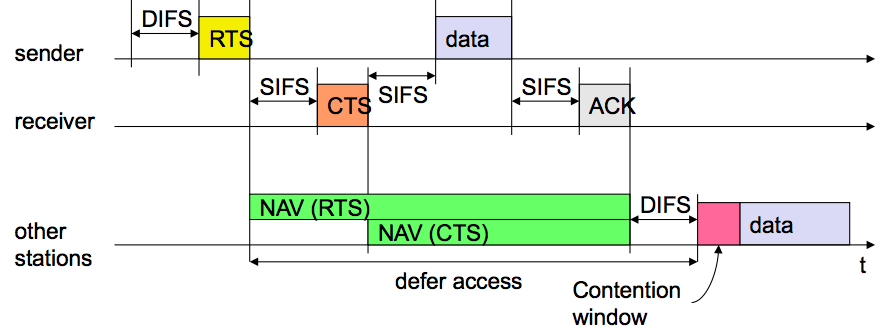
\includegraphics[width=7cm]{img/cdma_timeline}
\end{Figure}

\begin{Figure}
  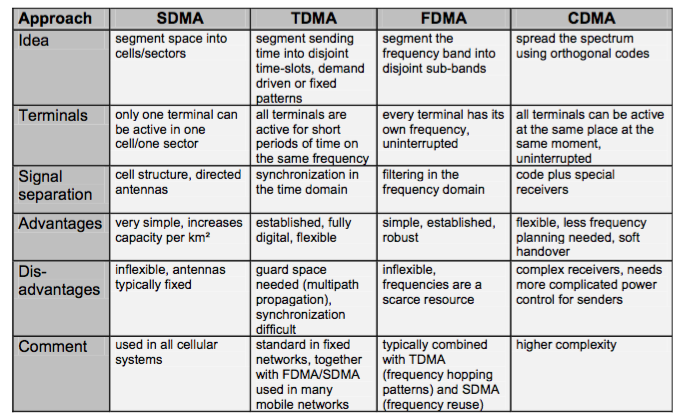
\includegraphics[width=7cm]{img/contentionfree}
\end{Figure}

\begin{Figure}
  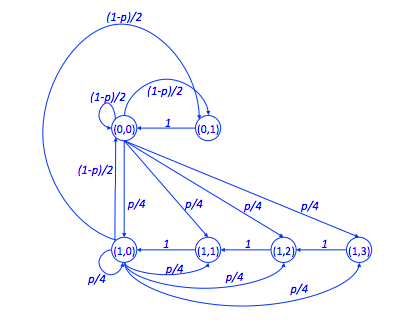
\includegraphics[width=7cm]{img/banchi.png}
  Bianchi model with 6 steates in total. $p$ denote the probability that collision happens
\end{Figure}
\end{multicols*}


\end{document}